% \documentclass[tikz,convert={outfile=\jobname.svg}]{standalone}
\documentclass[tikz,convert=pdf2svg,border=20pt]{standalone}
%\usetikzlibrary{...}% tikz package already loaded by 'tikz' option
\usetikzlibrary{arrows, arrows.meta}
% \tikzset{
%   >=stealth',
% }

\usepackage{amsmath,amssymb}
\usepackage{ndtheme}

\begin{document}
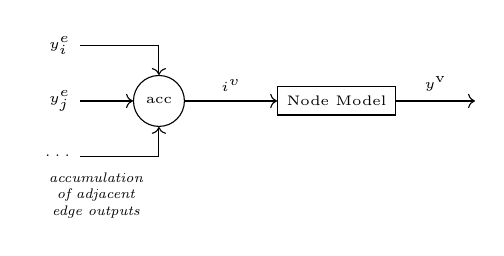
\begin{tikzpicture}[\ndtheme]
  % Write "Node model"
  \node[draw, font=\tiny](n){Node Model};

  % Write y^v
  \draw[->](n.east)--++(1.0,0) node[above, pos=.5, font=\tiny]{$y^{\mathrm v}$};

  % Draw the accumulator circle
  \node[font=\tiny, draw, circle] (acc) at ([xshift=-1.5cm]n.west) {$\mathrm{acc}$};

  % Connect acc to the node
  \draw[->] (acc) -- (n.west) node[above, pos=.5, font=\tiny]{$i^{v}$};

  % Add three arrows to acc with rectangular corners and write y^e_i, y^e_j and ...
  \draw[<-] (acc) |- ++(-1.0,0.7) node[left, font=\tiny](in){$y^e_i$};
  \draw[<-] (acc) -- ++(-1.0,0) node[left, font=\tiny]{$y^e_j$};
  \draw[<-] (acc) |- ++(-1.0,-0.7) node[left, font=\tiny]{$\ldots$};

  % Add a label for the accumulation function
  \node[text width=1.5cm, align=center, font=\itshape\tiny] at ([xshift=-0.8cm, yshift=-1.2cm]acc) {accumulation of adjacent edge outputs};
\end{tikzpicture}
\end{document}